\chapter{Memory}

\section{RAM access time}
In this part, we report latency for individual integer accesses to main memory and the L1 and L2 caches.

\paragraph{Methodology}
To test memory access latency, I first followed the procedure described in the lmbench paper \cite{ramacc}, testing different stride lengths over varying sizes of arrays. 

Then I did not use normal array access, like A[i]. Because it may have other overheads. For example, the compiler may first calculate the address then access the element. Instead we use pointer access and store the next pointer in current variable. So we allocate an array of pointer of int, and each store the next element address.

\paragraph{Predictions}

\pagebreak

\begin {figure}
\centering
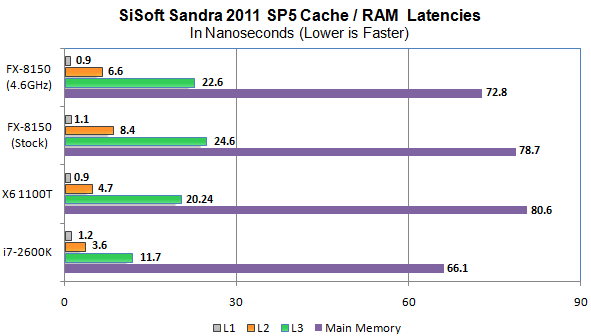
\includegraphics[width=6in]{./pics/Sandra-Latency.png}
\caption{RAM access speed reference}\label{RAM access speed reference}
\end{figure}

From Figure 4.1, we can see that different level caches and main memory have different speed.  Based on i7-2600k data, we made 20\% - 30\% improvement on this data and made following predictions : 

For L1-cache, we predict hardware overhead are 5 cycles and software 2 cycles;
For L2-cache, we predict hardware overhead are 10 cycles and software 4 cycles;
For L3-cache, we predict hardware overhead are 15 cycles and software 6 cycles;
For main memory, we predict hardware overhead are 90 cycles and software 60 cycles;

\paragraph{Results}
We present our measure results.

\begin {figure}
\centering
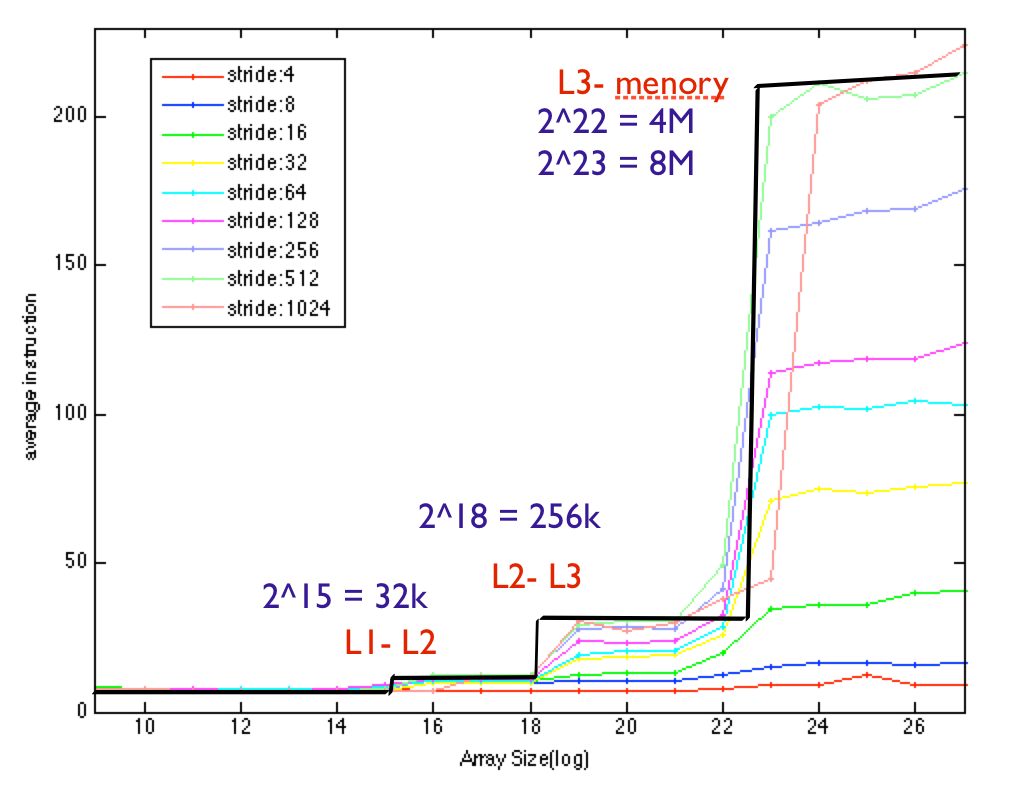
\includegraphics[width=2.6in]{./pics/ram1.png}
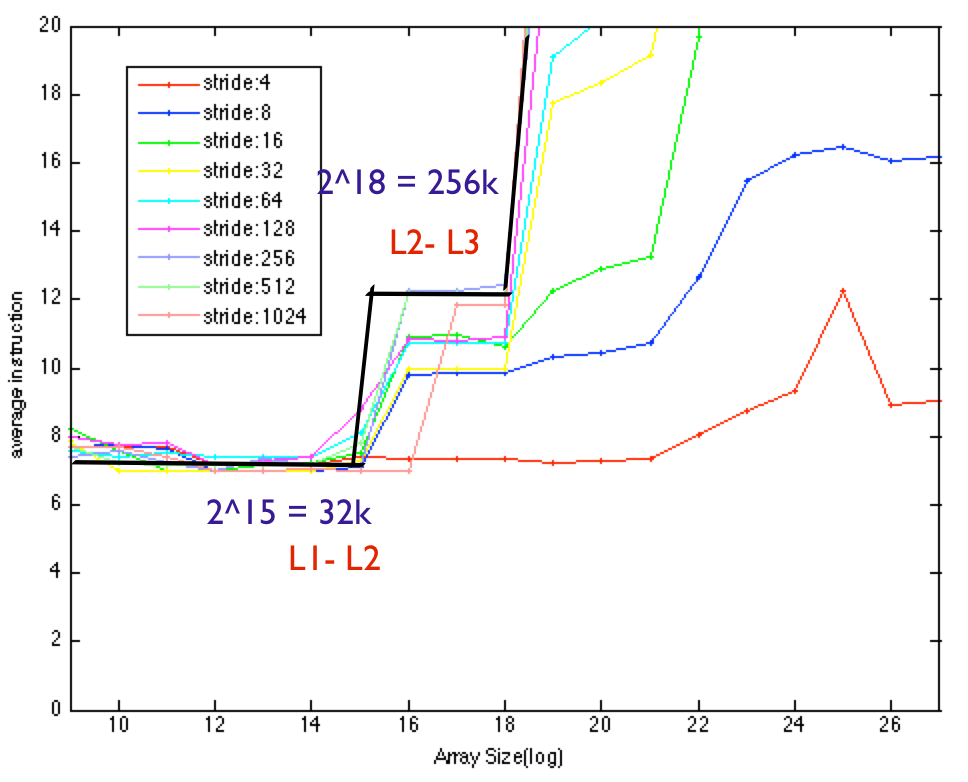
\includegraphics[width=2.6in]{./pics/ram2.png}
\caption{RAM access result}\label{RAM access}
\end{figure}

\begin{center}
\begin{tabular}{| p{1.5cm} | p{2cm} | p{2cm} | p{2cm} | p{2.5cm} | p{3cm} | p{2cm}}
TYPE             & Hardware  & Software  & Overall  & Measured  & Remove Overhead & Std\\
\hline

L1	&   5 cycles  & 2 cycles & 7 cycles  &  7.5  cycles &  4.5 cycles & 0.1212\\
L2    &   10 cycles & 4 cycles & 14 cycles & 11.2 cycles &  8.2 cycles & 0.2059\\
L3 	&   15 cycles & 6 cycles & 21 cycles &  24.2 cycles & 21.2 cycles & 0.4529\\
Memory & 90 cycles & 60 cycles & 150 cycles & 200.3 cycles & 197.3 cycles & 6.2800\\
\end{tabular}
\end{center}

\paragraph{Discussion}
Our prediction is very close to the measured result, it is due to the i7-2600k data. The data is very accurate, so we made good predictions on top of this data.

It is easy to see the transition from L3-cache to main memory, it is very steep in the picture from array size 22 to 23. Because my L3-cache is 6MB, so it is between 22 and 23.

We can also see the transitions from L2-cache to L3-cache. In the picture exactly in 18, the access time increase. Because my L2-cache is 256KB, which is equal to 18 in the picture.

In the scaled picture, it is very obvious to see transition from L1-cache to L2-cache, located in 15(32K).

We can also see that within cache, the RAM access time cycles are very small compared to that of main memory access.



\section{RAM bandwidth}
In this part, we report bandwidth for both reading and writing.

\paragraph{Methodology}
First, we create an array of size 32 MB that is bigger than L3-cache(6MB) and can be put into memory. In order to reduce the effects of cache line prefetching, we access array as follow : $0 -> HALF\_SIZE -> 1 -> HALF\_SIZE+1 -> ... -> ...$.  But this method can not totally remove the effect of cache line prefetching, because other cache line may cache different parts of the array.

To further reduce the overhead, we apply loop unrolling. Compared with code that did not apply loop unrolling, the bandwidth increased  a lot.

\paragraph{Predictions}

I found an estimation about different RAM\cite{ramref}.

\begin{figure}[!htb]
\centering
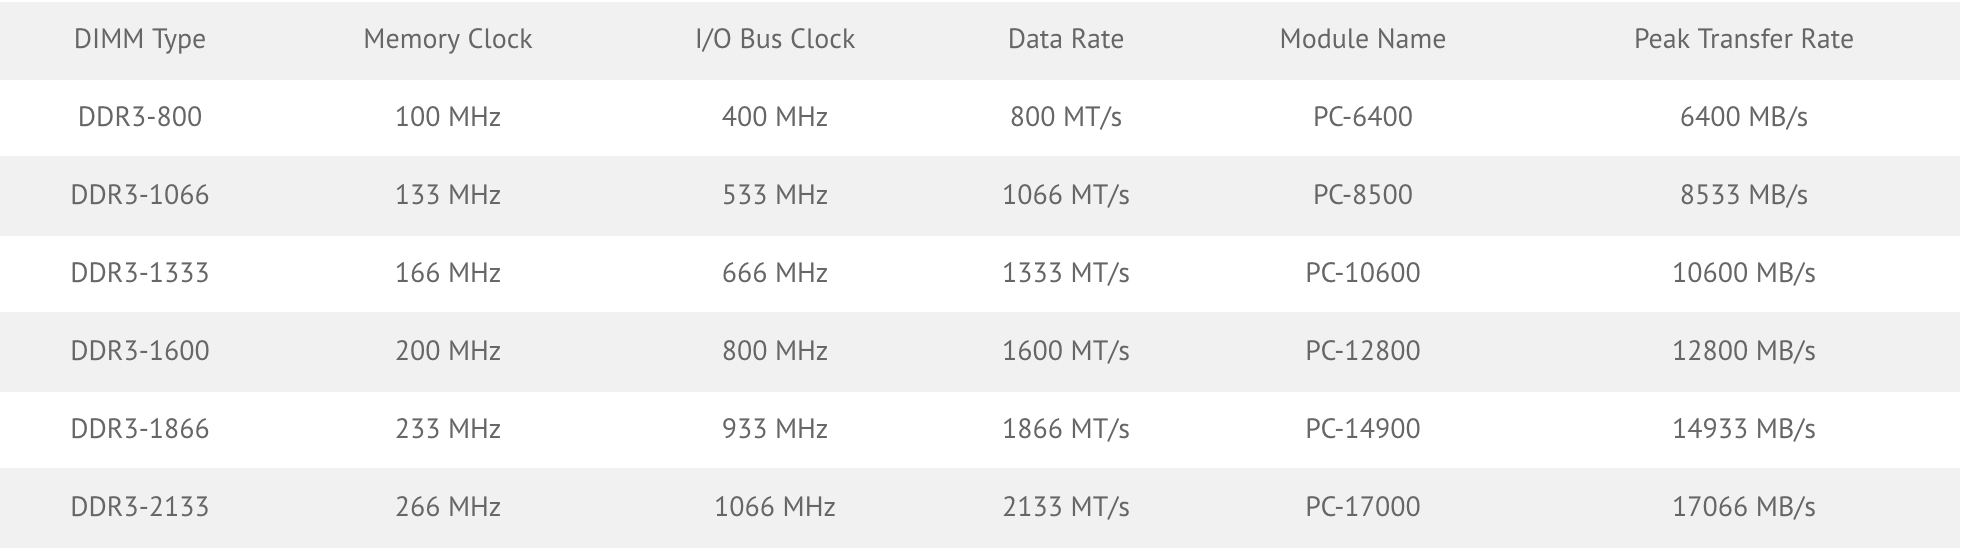
\includegraphics[width=6in]{./pics/ram_ref.png}
\caption{RAM bandwidth}\label{RAM bandwidth}
\end{figure}

According to this article and my memory : 1600 MHz DDR3. the bandwidth of my machine should be 12800 MB/s. 

\paragraph{Results}
We present our measure results.

\begin{center}
\begin{tabular}{l*{6}{c}r}
Operation             & Predicted Speed & Measured Speed & Std \\
\hline
READ & 12800MB/s & 8754MB/s & 99.49 \\
WRITE & 12800MB/s & 6902MB/s & 92.45\\

\end{tabular}
\end{center}

\paragraph{Discussion}
The prediction is a little higher than our measured results. 

Our method has eliminated the effects of cache line prefetching and use loop unrolling to reduce iteration overhead. That's why we choose 32MB array. Because an array of this size can not be put in cache totally and we can access array to make cache miss.

One of the drawback of our method is that we access each element of small size, which may include some overhead. If I have a big struct or class, maybe we can get higher results. 

And write speed is less than read speed, I think it is due to the read prefetching. Because different cache line may cache different parts of my array.

\section{Page fault service time}
In this part, we report the time for faulting an entire page from disk.

\paragraph{Methodology}
According to the hint, we find that mmap is one useful mechanism. Because file contents are not read from disk initially and do not use physical RAM at all. The actual reads from disk are performed in a "lazy" manner, after a specific location is accessed. Before accessing the content, we record time, after accessing we record again then we can get the page fault service time.

\paragraph{Predictions}
According to some OS textbook \cite{page}, the page fault service time is about 8ms, the CPU frequency at that time is about 5MHz. So 8ms is about 16000 cycles.

Because my page size is 4 KB, every page fault will loading 4 KB data from disk to memory. SSD read/write speed is fast, so I predict the hardware overhead are 4096 * 2 = 8192 cycles and software overhead are 8000 cycles.

\paragraph{Results}
We present our measure results.

\begin{center}
\begin{tabular}{| p{2cm} | p{3cm} | p{3cm} | p{2.5cm} | p{2.5cm} | p{2cm} }
Operation  & Base Hardware Performance  & Estimated Software Overhead  & Predicted Time  & Measured Time  & Std \\
\hline
Page Fault Service Time & 8192 cycles& 8000 cycles& 16192 cycles& 8528 cycles & 11.33405\\

\end{tabular}
\end{center}

\paragraph{Discussion}
Our estimation is a little higher than the measured result. Maybe today  the linux kernel serve page fault faster than that time or the hardware is much faster. For example, it is much faster to read a page via SSD than HDD.

Whenever the cpu detects a page-fault, its action depends on Current Privilege Level. If  CPL == 3  (executing in user mode)
the CPU will switch to its kernel-mode stack:

\begin{enumerate}
\item push  SS  and  ESP
\item push  EFLAGS
\item push  CS
\item push  EIP
\item push  error-code
\item jump to the page-fault service-routine  
\end{enumerate}

So there are a lot of work to do. 


\paragraph{Question} Dividing by the size of a page, how does it compare to the latency of accessing a byte from main memory?

The page size in our system is 4 KB, so it is approximately 1-2 cycles per byte of data transfered, compared to about 200 cycles per byte from main memory. May be this is the power of SSD.
